\chapter{Languages}
\label{languages}
The preceding section described a representation for programs which is suitable for any language. To define a particular language in this framework involves defining three aspects of the language.

The \emp{abstract syntax} of the language defines what nodes may appear in a program, and in what relationship to each other. In \Meta, abstract syntax is defined by a program in the \keyword{grammar} language. The grammar program is first and foremost a specification which defines what programs are (syntactically) valid. 

Every language must have a \emp{semantics} that gives its programs meaning. While there are any number of ways to specify semantics, or indeed to make use of languages and programs with only ill-defined semantics, the approach pursued here is that of one or more kernel languages and syntax extension. The example of Lisp shows this to be a successful strategy, so the experimental question is how well it applies in this new setting. When a grammar defines a node type, it may also define the semantics of the construct by means of a reduction to a more primitive construct.

With abstract syntax and semantics taken care of, both the Lisper and the Programming Language Theorist have all they need and will go happily on their ways. However, we would like to go further than that, so one more element is needed. \emp{Concrete syntax} is what the user reads and writes. The goal is to take advantage of the new approach to do things with concrete syntax that are impractical or impossible to do with textual source code. In \Meta, the concrete syntax of each type of node is given as a reduction to a \emp{presentation language}.

%
% Grammars
%
\section{Grammars}
\label{grammars}
Thus the grammar defines all three aspects of the language. The abstract syntax is defined \emp{prescriptively}, by determining what programs are legal. Both the semantics and concrete syntax are defined \emp{operationally}, as declarations of what reduced program and what visual representation will be derived from each source node.

\subsection{Abstract Syntax}
A program is \emp{valid} with respect to a \emp{grammar} if all of its node's types, values, and references comply with certain restrictions imposed by the grammar. For each node type, a grammar specifies:
\begin{enumerate}
\item Zero or more \emp{abstract types}, which are types for which the type being introduced is a \emp{sub-type}.
\item Whether the node's value should be an boolean, integer, string, sequence, or map.
\item For an integer-valued node, a range of legal values.
\item For a sequence node, the number and (abstract) type of expected child nodes.
\item For a map node, the expected attributes and the (abstract) types of nodes that may inhabit each of them.
\item When a child/attribute is a reference, the type of the expected (abstract) type of the referenced node.
\end{enumerate}

Abstract types lend some modularity to the grammar. A new subtype of any abstract type can be introduced later without changing any existing definition, and nodes with the new type can appear as children of nodes of the previously-defined types. Note: these simple types are entirely nominal---there is no inheritance of any kind, the type is meant exclusively to record the intended meaning of each node, and to guide the grammar in applying the rules of the abstract syntax.

Note that all these properties except the last are local in the sense described earlier---checking them requires inspecting only a single node and its immediate children. Checking the type of the node pointed to by a reference requires being able to inquire about the type of a node which may be anywhere in the program. However, this information is easily extracted up front to a map of types for all nodes in the tree, so this one non-local check seems to be worth including in the standard checker.

A grammar so-defined is not capable of specifying every interesting property of a language. That is, not every syntactically valid program is correct. Depending on the nature of the language being defined, additional, more ambitious specifications can define additional properties (e.g. proper use of lexically-scoped variables or type safety). The abstract syntax is meant to be an easily-defined first step, and indeed in some sense it \emp{is} the language (e.g. a Java program with type errors is just that, but a program that fails to adhere to the basic syntactic structure of Java doesn't seem to rate being called a Java program at all.)


\subsection{Reductions}
A grammar may supply one or two reductions for each node type. These reductions are code fragments which are used to construct reduction functions (see section \ref{reduction}) which take a program in the source language defined by the grammar and reduce it to a derived program. Using a meta-programming approach, the reductions are economical and simple to define, but the full host language is available for use in reductions when needed. %See Figure \ref{fig-and}.

\begin{figure}[ht]
%  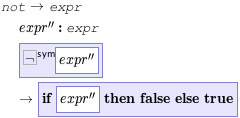
\includegraphics[scale=0.8]{src/image/not.png}  % 72dpi/0.8 = 90dpi for display

  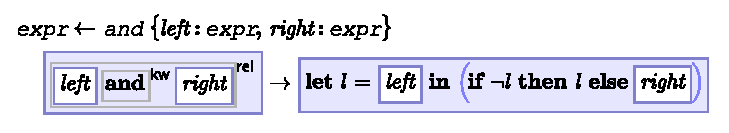
\includegraphics{src/image/and.pdf}
  \caption[Declaration of the \keyword{and} node of the core language.]{Declaration of the \keyword{and} node, taken from the grammar for the \Meta\ core language. \keyword{and} is an subtype of the abstract type \keyword{expr}, has two required attributes, \emp{left} and \emp{right}, both \keyword{expr}s. It is displayed with the infix keyword ``and'', and reduces to an expression using the primitives \keyword{let} and \keyword{if}.}
  \label{fig-and}
\end{figure}

A \keyword{display} reduction (shown on the left in Figure \ref{fig-and}) reduces a node to a presentation language node. This reduction will always be present except in certain special cases which will be described later.

An \keyword{expand} reduction is used to reduce a node in preparation for evaluation or execution, and therefore defines the semantics of the node. The result of this reduction is either a node in the \emp{target language}, or else a node that will itself be reduced, eventually to a target language node. The declaration of a node type does not provide an \keyword{expand} reduction if the node's semantics is defined externally; in that case the un-reduced node is already in target-language syntax.

It is easy to define a reduction that fails to terminate (by producing a node of equal size), or which ``blows up'' (by producing a larger, but no more reduced, node). However, this is mostly a problem in the early stages of language definition when core constructs are being defined on top of one another; once a usable core is available, most extensions build on that in a simple way. Anyway, once language definition is part of the development process, it should no longer be so surprising that problems can arise at that level. Because you are your own language vendor, you can simply fix it; it's not like finding a bug in your C++ compiler, which you may have no capability to fix.

Thus the abstract syntax, semantics, and concrete syntax of every language construct are defined together in a simple, declarative style. Therefore, each language construct is self-documenting. This flavor will be maintained in more interesting examples to come.

%
% Kernel languages:
%

\section{Kernel Languages}
A \emp{kernel language} is one whose nodes have some fixed, pre-defined semantics (typically, they can be evaluated, yielding some specified result with some specified side effects). A complete language is built by \emp{extending} a kernel language with additional nodes whose semantics is defined in terms of reduction to (ultimately) the kernel language.

Any language can act as a kernel language in \Meta. If the kernel language is of a more conventional type, say Java, all the constructs of that language have to be defined as primitives. Additional constructs could then be defined via reduction to ordinary Java syntax. After reduction, the target program would be processed by a Java compiler to produce an executable. Thus a language like Java is a suitable kernel language, but hardly a convenient one.

One kernel language, the \emp{host kernel language}, is designed to be much more simple to implement and use. It is the glue that makes the system work; for example the reductions themselves are written in it. Requirements for the host kernel language include:
\begin{enumerate}
\item Be in some sense minimal but sufficient, so that everything else can be done via extensions of it.
\item Be a meta-language, able to consume and produce nodes.
\item Fit well with the ``functional'' approach to nodes and trees.
\item Be easily implemented and easily integrated into a running application.
\end{enumerate}

In section \ref{host}, we'll describe the host kernel language of \Meta\ and how it fulfills these requirements.

The idea of a very minimal kernel language with a core language built on top of it is of course inspired by the Lisp family of languages. In particular, in Scheme\cite{scheme}, only a handful of \emp{special forms} are pre-defined, and all other language constructs are defined ``in the language'' in terms of macros which expand into the special forms. A similar approach is used for more didactic purposes in Mozart\cite{mozart}, at least in \emp{defining} the language, although it isn't clear that the implementation actually works this way.

%
% Presentation languages:
%

\section{Presentation Languages}
The nodes of a \emp{presentation} language cast program elements in visual terms. A presentation language should be independent of the particular syntax of any one language, but might be suited to a particular family of related languages. Crucially, the presentation language must be flexible enough to represent any conceivable construct that might be added to the source language. This is achieved by providing composable elements in the presentation language that can be combined in new ways to create new concrete syntax.

A presentation language is concrete in that it represents the program as it is presented to the user, however it is somewhat abstracted from the details of rendering characters and pixels. The reduction from source to presentation language is therefore quite direct and simple. Once the program is reduced to the presentation language, lower-level processing takes care of the details of rendering. This lower-level processing is common to all languages using the same presentation language, and does not need to be extended in the typical course of using (and extending) a source language.

To serve the needs of different kinds of languages, multiple presentation languages could be defined, such as a ``flowing text'' language for documents, a ``grid'' language for spreadsheet-like programs, a ``flowchart'' language for state machines, data flow programs, and regular expressions, and so forth. In \Meta, a single presentation language is currently implemented.

\subsection{The \keyword{expr} Language}

%\begin{figure}
%\todo{capture from the implementation}
%$$\keyword{keyword} = \mathit{str} : \keyword{string}$$
%$$\keyword{int} = \mathit{str} : \keyword{string}$$
%$$\dots$$
%\caption{\label{fig-expr} Grammar for the \keyword{expr} language.}
%\end{figure}

\Meta's \keyword{expr} language is well-suited to representing the expressions that make up the declarative portion of a typical modern programming language and it can also reproduce much of the familiar notation of algebraic expressions. An \keyword{expr} program is a tree made up of \emp{box} nodes. Each box node occupies a rectangular area of the rendering surface and always encloses the areas occupied by any child boxes. Several kinds of boxes are available in \keyword{expr}.

An \emp{atom} is a box that renders a sequence of characters and/or symbols using the normal spacing for text. Several types of atoms are available, each conveying what kind of entity the characters are meant to represent. When atoms are reduced to lower-level nodes, a distinctive typographical treatment is applied to each, as shown in Table \ref{fig-atoms}. The list of atom types is meant to be expanded to serve the needs of any conceivable source language; the effort to add a new type is typically small (most simply specify a font and/or face), and in any case the total number of types in any one language is probably limited to a dozen or so, with much in common across languages, so we conjecture that the universe of useful atom types is not much larger than what \keyword{expr} currently provides. 

\begin{table}
\begin{tabular}{llll}
Type & Treatment & Examples & Typical use
\\
\hline
\keyword{keyword}
 & boldface
 & \keyword{true}
 & fixed language syntax
\\ & & \keyword{if} &   % Ugly hack! how to do proper multi-line cells in tabular env.?
\\
\hline
\keyword{var}
 & italic
 & $x$
 & names (user-provided or generated)
\\ & & $g$ & 
\\ & & $\mathit{fib}$ & 
\\
\hline
\keyword{num}
 & \textit{none}
 & 1
 & numerical literals
\\ & & 2.0 & 
\\ & & 3,000 & 
\\
\hline
\keyword{string}
 & sans serif
 & \textsf{abc} 
 & character literals (note special
\\
 & & \textsf{Hello,\textvisiblespace world} &  % open box: \u2423
  treatment of the space character)
\\
%\hline
%\keyword{name}
% & boldface, italic
% & \textbf{\emp{a}}
% & name literals
%\\ & & \textbf{\emp{foo}} & 
%\\
\hline
\keyword{mono}
 & monospaced
 & \texttt{nil}
 & external references
\\ & & \texttt{cons} & 
\\
\hline
\keyword{prod}
 & monospaced, italic
 & \texttt{\emp{expr}}
 & node types in grammars
\\ & & \texttt{\emp{left}} & 
\\
\hline
\keyword{symbol}
 & \textit{none}
 & $\to$
 & mathematical symbols
\\ & & $\in$ & 
\\ & & $\sum$ & 
\\
\hline
\end{tabular}

\vspace{6pt}

\caption{Types of atoms in \keyword{expr}, and the typographical treatment that is applied to them when \keyword{expr} is reduced. Note: the actual character content of each type of atom is arbitrary, except \keyword{symbol}, which provides a pre-defined set of available symbols.}
\label{fig-atoms}
\end{table}

The diversity of atom types provides a measure of visual sophistication for programs, with a very small effort on the part of the language designer. Simply by identifying a visual style for each piece of syntax, some information about the meaning of each node is conveyed to the programmer. The particular treatment is meant to match the readability and high aesthetic standards of the pseudocode that might be found in a journal article or a good CS textbook.

A similar idea leads to the \emp{syntax-coloring} behavior of many text editors, with a more cartoonish and less elegant result (see Figure \ref{fig-syntax-coloring}). In \Meta, using a single color for all syntax allows color differences to be used for other purposes.

\begin{figure}[ht]
  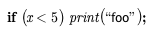
\includegraphics[scale=0.8]{src/image/if.png}
  
  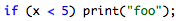
\includegraphics[scale=0.8]{src/image/if-text.png}

  \caption{\label{fig-syntax-coloring}Comparison of visual rendering of a simple Java expression, at 90 dpi. }
\end{figure}

\emp{Composite} boxes contain child boxes which they arrange in a certain way. A \emp{sequence} is a horizontal arrangement of nodes separated by a certain amount of space. There are a handful of sequence types, each implying a certain amount of inter-node space. The amount of space is a visual indication of how tightly the sub-expression represented by the sequence binds, as we'll discuss in the next subsection. A \keyword{scripted} node contains a \emp{nucleus} and one or both of a \keyword{sub}- and \keyword{super}-script node. \emp{Special signs} are similar to composites but also draw a glyph surrounding the child node(s). Examples are \keyword{radical} and \keyword{fraction}, used in particular mathematical contexts.

A \keyword{group} node draws a pair of grouping symbols around a content node. Available symbols include parentheses, various kinds of brackets, $\lfloor\mathit{floor}\rfloor$, $\lceil\mathit{ceiling}\rceil$, and $|\mathit{magnitude}|$. All these symbols expand vertically to visually surround their contents; this variation is aesthetically pleasing, but also provides a visual cue which helps the reader to match up the paired symbols.

An \keyword{embed} node encloses its contents in a visual indication of being a separate unit, contained within the surrounding context. A \keyword{disembed} node has the opposite effect, showing its contents as being part of the outer level of code. These are used in the rendering of quotations, and have been seen already in the example reductions in Figure \ref{fig-and}.

Because the \keyword{expr} language preserves the hierarchical structure of expressions and specifies the visual layout of each sub-expression, it's possible for the system to identify cases where the nesting of expressions could lead to confusion, and to insert parentheses automatically in these cases. This is done \emp{after} the reduction of the program to the \keyword{expr} language, so it's applied consistently to any language construct, without special effort at the point of definition of a node. 

The \keyword{expr} language provides enough levels of spacing (four) to handle a moderately complex expression without parentheses. For example, in the expression\begin{center}
%$$\keyword{if} \:\ \: x \: < \: y + 4! \:\ \: \keyword{then} \:\ \: \dots$$ 
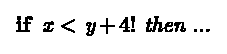
\includegraphics{src/image/space.pdf}
\end{center}
% too much space here!
the factorial operator binds most tightly ($!$, no space), then addition is performed ($+$, indicated by a thin space), then comparison ($<$, medium space), and finally the conditional (\keyword{if}, thick space). Examples of how this works will be presented later.



\keyword{expr} provides no real support for sequences of statements, or for larger constructs such as methods, classes and modules. These larger constructs pose different layout problems, such as how to handle indentation and whether lines should be wrapped and how. Therefore, it would make sense to implement a second presentation language, say \keyword{program}, which would include nodes for these concepts. In \Meta, these constructs can be implemented somewhat awkwardly using the lower-level presentation language described in section \ref{view}.

%
% Extending...
%

\section{Extending a Language}
The grammar language, host language, and presentation language work together to support the definition of new language constructs. A grammar (i.e.\ a program in the \keyword{grammar} language) consists of a collection of node type declarations (\keyword{grammar} nodes), each containing reductions (which are host language nodes). A display reduction in turn contains quoted nodes in a presentation language (e.g.\ \keyword{expr}), while an ``expand'' reduction quotes nodes in the target language (which may be the host language or some other target language). This is only the start; a grammar can define syntax for embedding subtrees in yet more languages, such as when a regular expression sub-language is added as an extension to a general-purpose language. This extensive embedding is the key to economy of expression in \Meta.\footnote{And it inspired the name \Meta. A grammar is a meta-language, so the grammar for grammars is a meta-meta-language. Warning: this kind of thing is fun when it works, but it can be a mind-twisting chore to get it bootstrapped.}

\temp{When it's desirable to keep track of what source node gave rise to a given target node, the reduction can record the labels of each pair of source and target node, forming a kind of mapping between the parallel trees. For this to work, the reduction function needs to operate strictly on the single node it's given, and not reach into any child node. This in turn places some constraints on the way the source program is constructed: each node (along with any environment) must bear sufficient information to identify the correct reduction.}

Because a grammar is a \Meta\ program, the same tools for syntax extension are available for use in grammars, so the \keyword{grammar} language should be viewed as a starting point. It is meant to be general enough to define typical languages, to handle most common needs for defining syntax, and to serve as a kernel language for grammars.

As an example, consider the variety of binary infix operators that we may wish to define. If defined in terms of the kernel grammar language, each declaration will echo the definition of \keyword{and} shown in Figure \ref{fig-and}, varying only in the symbol used to represent the operator, and the name of the function to invoke (assuming many of these are simply wrapping some primitive operation supplied by the platform). This kind of duplication is a clear opportunity for language extension, as shown in Figures \ref{fig-binary} and \ref{fig-binary-examples}.

\begin{figure}[h]
  \todo{capture: binary \{ type: name, symbol: name, fn: string \} xxx $\to$ [expr $\leftarrow$ [name] ...]}
  
  \caption{Definition of the \keyword{binaryNode} extension to the grammar syntax.}
  \label{fig-binary}
\end{figure}

\begin{figure}[h]
  \todo{capture: plus, minus, in, :, ++, ?, \%}
  
  \caption{Some infix operators defined using \keyword{binaryNode}.}
  \label{fig-binary-examples}
\end{figure}

Note that the presentation for the new node visually approximates the original declaration, but it is in fact much simplified. This simplification becomes apparent when you edit one of these nodes---only the three unique elements can be edited, and the rest of the visualization is provided by the reduction. Like much syntax extension, the new node embodies the well-known Don't Repeat Yourself principle\cite{dry} by eliminating code duplication. Still, the meaning is clear at a glance because the presentation supplies cues which are easily recognized by their visual resemblance to the lower-level form.

%\section{JUNK: More Stuff}

%\subsection{Parentheses}
%Of particular interest is the handling of parentheses. At the AST level, it is never necessary for the programmer to use parentheses to make the meaning of an expression clear, because the intended order of operations is explicit in the structure of nodes. However, some indication of grouping may be needed at the presentation level to produce an unambiguous visual representation. In \Meta, these parentheses are introduced automatically after the program is reduced to the \keyword{expr} language. 

%Thus the role of parentheses is turned around: instead of being provided by the programmer as a hint to the parser about how the expression should be constructed, they're provided by the system, as a form of feedback to the programmer about the structure of the program that's being written/read. \temp{...reflects the reality of the programmer/editor interaction, which is about iteratively making edits and then reading the resulting text -- it's not a question of coming up with the program in your head and then typing it out in a stream.}

%The insertion of parentheses is handled in a language-independent way, taking advantage of the way expressions are represented in the \keyword{expr} language. Pairs of parentheses (in the form of a \keyword{delim} node) are inserted around a sequence if it is nested within another node in such a way that the resulting notation would otherwise be misleading. By taking over the notational details, \Meta\ relieves the programmer of a sometimes tedious task, but more importantly ensures that the visual form of the program always corresponds closely to the actual meaning.

%For example, consider the following pair of related expressions:
%$$n! - 1 \qquad \qquad \qquad \lsyn n - 1 \rsyn !$$
%In the first expression, $n$ factorial is calculated first, and then 1 is subtracted from that. The tighter binding of the factorial operation is visually suggested by the juxtaposition of $n$ and $!$ with no space between. The second operation is displayed with thick spaces interposed, suggesting looser binding. Thus the visualization matches the expression's structure without any additional fuss. In contrast, in the second expression, the usually tighter-binding operation is performed second, so a pair of parentheses is inserted around $n-1$ to indicate the proper order. 

%A handful of simple rules determine when parentheses are inserted, depending on the type of the parent and child node, and a few special cases (for example, a \keyword{nucleus} needs parens, but \keyword{super} and \keyword{sub} nodes do not). Figure \ref{fig-parens} shows several additional examples that cover most of the cases\footnote{Knuth in the TeXbook (p.\:140): ``\dots takes a bit of mathematical knowhow, since parentheses sometimes need to be inserted in order to preserve the meaning of the formula\dots If you are a typist without mathematical training, it's best to ask \dots for help.'' If Knuth had implemented this algorithm, his typists would have been spared this chore. However making the process manual does give the author a greater degree of control, which is probably appropriate in the context of publishing.}.

%
%\begin{figure}[ht]
%\todo{use my own output, which will be a better demonstration anyway}
%$$
%\begin{array}{ccc}
%\lsyn 1+2 \rsyn \!\cdot\!3 & 
%  \mathrm{\it vs.} & 
%  1 + 2\!\cdot\!3
%\\
%\vspace{6pt}
%\\
%{\lsyn x+2 \rsyn}^i &
%  \mathrm{\it vs.} & 
%  x^{i+2}
%\\
%\vspace{6pt}
%\\
%{\lsyn a+b \rsyn}/2 & 
%  \mathrm{\it vs.} & 
%  {{a+b} \over 2}
%\\
%\vspace{6pt}
%\\
%{\lsyn y-1 \rsyn}^{1/2} + 2 & 
%  \mathrm{\it vs.} & 
%  \sqrt{y-1} + 2
%\end{array}
%$$
%\caption{Examples of expressions that require parentheses (on the left), and related expressions where the notation is unambiguous and no parentheses are needed (on the right). Note that in cases where the meaning is equivalent, one or the other form might be preferable from an aesthetic point of view, but the transformation from one to the other is not necessarily trivial (see footnote). All examples are output from \Meta, with parentheses inserted automatically.}
%\label{fig-parens}
%\end{figure}

%From the point of view of the language-definer, the impact is that there's no need to define or to document rules about operator precedence; you simply supply the desired notation. The \keyword{expr} language provides enough levels of spacing (four) to handle a moderately complex expression without parentheses. For example \todo{use actual output?}:
%$$\keyword{if} \quad x \: < \: y + c! \quad \keyword{then} \quad \dots$$
%Contrast this with textual languages: C has about 15 fixed precedence levels for its infix operators, C++ has 18, and Haskell allows new operators to be defined at any of 9 levels. This apparent bounty is misguided; it allows the programmer to avoid a little typing but is a ``notorious source of bugs''\cite{realworldhaskell} when the compiler and human reader don't agree on an expression's meaning.

%% ``Even more importantly, complex expressions that rely completely on operator precedence are notorious sources of bugs. A compiler and a human can easily end up with different notions of what even a short, parenthesis-free expression is supposed to do.
%%``There is no need to remember all of the precedence and associativity rules numbers: it is simpler to add parentheses if you are unsure.'' - Real World Haskell

%

%\subsection{Embedding (Quotations) [todo]}

%\temp{how embedding makes meta-programs comprehensible}

%\temp{dual interpretation: code vs. visual template}

%\temp{example of a presentation reduction with a conditional first? n-ary AND?}

%
%\subsection{Names [todo]}
%Another element of programs that gets special treatment 

%

%\section{ASTs at Runtime}\todo{}

%\temp{how much is there to say here? leave it to example 3?}

%
%\temp{random comment: Note that grammars are currently defined as discrete programs, but in a real language the grammar might be constructed as the program is loaded and syntax declarations are processed.}

%%
%%
%%

%
%By contrast, in a conventional language the concrete and abstract syntaxes are defined implicitly by the parser, and the semantics is defined somewhere inside the compiler. If there's any documentation, it has to be produced by a separate effort\footnote{If a \emp{parser generator} is used, then it may be able to produce some documentation of the syntax from the grammar. However in practice this kind of generated documentation tends to be difficult to use, due to the relative complexity of grammars that are meant to be used for parsing.}.


%\subsection{Extending the Grammar Language}
%Because a grammar is a \Meta\ program, the same tools for syntax extension are available for use in grammars, so the \keyword{grammar} language just described should be viewed as a starting point. It is meant to be general enough to define typical languages, and to handle most basic common needs for defining syntax. There are a couple of ways this language could be extended to provide additional power.

%Using syntax extension, new kinds of node declarations could be supported. For example, an \keyword{infix} node declaration would require only an operator symbol and an expression to evaluate given two arguments. It would reduce to a declaration of a sequence node type,  requiring 2 or more argument expressions, a presentation reduction taking care of interposing the operator, and a left-to-right reduction of the arguments. \todo{actually, that would be awesome. should I implement it?}

%Going further, a richer grammar language could provide additional specifications which would be consumed by a new checker. An example would typing rules. In this case, the enriched grammar would be reduced to the \keyword{grammar} language by discarding the extra information.

